\documentclass[../main.tex]{subfiles}
\begin{document}
\counterwithin{figure}{section}
\counterwithin{table}{section}
\section{Additional tables}





\begin{table}[H]
    \centering
    \caption{Balance test (native)}
    \resizebox{\textwidth}{!}{\begin{tabular}[t]{lccccccc}
\toprule
  & Income (1,000) & Net wealth (1,000) & Oldest HH member (years) & Tenure (days) & Employed & Educ. length (years) & HH size\\
\midrule
New diff neighbor $k_{nearest}$ v $k_{near}$ & -1.408*** & -1.903*** & -0.043* & 1.936 & -0.002** & -0.035* & -0.009***\\
 & (0.254) & (0.402) & (0.020) & (5.999) & (0.001) & (0.014) & (0.002)\\
New diff neighbor $k_{near}$ v $k_{near}$ (omit.) &  &  &  &  &  &  & \\
 &  &  &  &  &  &  & \\
New diff neighbor $k_{close,10}$ v $k_{near}$ & -0.042 & 0.620 & 0.031 & 20.750*** & 0.001 & 0.010 & 0.005*\\
 & (0.255) & (0.402) & (0.019) & (5.710) & (0.001) & (0.013) & (0.002)\\
New diff neighbor $k_{close,20}$ v $k_{near}$ & 0.498* & 1.625*** & 0.109*** & 53.312*** & 0.002** & 0.025* & 0.015***\\
 & (0.224) & (0.377) & (0.018) & (5.262) & (0.001) & (0.013) & (0.002)\\
New diff neighbor $k_{close,30}$ v $k_{near}$ & 1.429*** & 2.993*** & 0.228*** & 93.723*** & 0.005*** & 0.045** & 0.029***\\
 & (0.256) & (0.402) & (0.019) & (5.823) & (0.001) & (0.014) & (0.003)\\
New diff neighbor $k_{close,40}$ v $k_{near}$ & 1.805*** & 4.979*** & 0.343*** & 124.422*** & 0.004*** & 0.055*** & 0.040***\\
 & (0.307) & (0.496) & (0.023) & (7.935) & (0.001) & (0.016) & (0.003)\\
\midrule
N & 5,365,811 & 5,365,811 & 5,365,811 & 5,365,811 & 5,365,811 & 5,365,811 & 5,365,811\\
Neighborhood-by-quarter FE & X & X & X & X & X & X & X\\
Mean of dependent variable & 341.26 & 60.61 & 44.05 & 2646.87 & 0.84 & 10.11 & 1.70\\
Number of neighborhoods & 3444 & 3444 & 3444 & 3444 & 3444 & 3444 & 3444\\
\bottomrule
\end{tabular}}
    \label{tab:balance_test_native_full}
    \begin{tablenotes}[flushleft]
\item \scriptsize * p < 0.05, ** p < 0.01, *** p < 0.001 \\ \textit{Note:} Standard errors (in parenthesis) are clustered at the municipality-year level. The table reports the estimate of $\phi_1 - \phi_3$ from equation \ref{eq:balance_tests}. 
\end{tablenotes}
\end{table}

\begin{table}[H]
    \centering
    \caption{Balance test (non-Western)}
    \resizebox{\textwidth}{!}{\begin{tabular}[t]{lccccccc}
\toprule
  & Income (1,000) & Net wealth (1,000) & Oldest HH member (years) & Tenure (days) & Employed & Educ. length (years) & HH size\\
\midrule
New diff neighbor $k_{nearest}$ v $k_{near}$ & -0.065 & 0.171 & -0.061* & 31.109*** & 0.001 & -0.011 & 0.001\\
 & (0.347) & (0.522) & (0.028) & (7.656) & (0.001) & (0.018) & (0.004)\\
New diff neighbor $k_{near}$ v $k_{near}$ (omit.) &  &  &  &  &  &  & \\
 &  &  &  &  &  &  & \\
New diff neighbor $k_{close,10}$ v $k_{near}$ & -0.075 & 0.514 & 0.064* & 58.269*** & 0.002 & 0.024 & 0.026***\\
 & (0.350) & (0.507) & (0.027) & (7.448) & (0.001) & (0.017) & (0.004)\\
New diff neighbor $k_{close,20}$ v $k_{near}$ & -0.315 & 0.400 & 0.191*** & 111.810*** & 0.001 & 0.021 & 0.039***\\
 & (0.319) & (0.467) & (0.026) & (6.707) & (0.001) & (0.015) & (0.004)\\
New diff neighbor $k_{close,30}$ v $k_{near}$ & -0.760* & 1.043 & 0.297*** & 157.738*** &  & 0.030 & 0.062***\\
 & (0.348) & (0.536) & (0.028) & (7.760) & (0.001) & (0.018) & (0.005)\\
New diff neighbor $k_{close,40}$ v $k_{near}$ & -1.064* & 2.171** & 0.430*** & 202.154*** &  & 0.013 & 0.064***\\
 & (0.455) & (0.700) & (0.037) & (10.536) & (0.002) & (0.023) & (0.006)\\
\midrule
N & 1,795,109 & 1,795,109 & 1,795,109 & 1,795,109 & 1,795,109 & 1,795,109 & 1,795,109\\
Neighborhood-by-quarter FE & X & X & X & X & X & X & X\\
Mean of dependent variable & 315.64 & 46.50 & 42.94 & 2298.84 & 0.84 & 12.11 & 2.11\\
Number of neighborhoods & 3,332 & 3,332 & 3,332 & 3,332 & 3,332 & 3,332 & 3,332\\
\bottomrule
\end{tabular}}
    \label{tab:balance_test_non_west_full}
    \begin{tablenotes}[flushleft]
\item \scriptsize * p < 0.05, ** p < 0.01, *** p < 0.001 \\ \textit{Note:} Standard errors (in parenthesis) are clustered at the municipality-year level. The table reports the estimate of $\phi_1 - \phi_3$ from equation \ref{eq:balance_tests}. 
\end{tablenotes}
\end{table}

\begin{table}[H]
    \caption{Estimate of Schelling behavior (native households)}
    \centering
    \begin{threeparttable}
        
    %\begin{adjustbox}{width=\textwidth, center}
        \begin{tabular}{lcccc}
\toprule
  & (1) & (2) & (3) & (4) \\ 
\midrule
New diff-type neighbor $k_{nearest}$ v $k_{close,20}$ & 0.949*** & 0.962*** & 0.747*** & 0.702*** \\ 
 & (0.097) & (0.098) & (0.090) & (0.077) \\ 
New diff-type neighbor $k_{near}$ v $k_{close,20}$ & 0.599*** & 0.601*** & 0.400*** & 0.379*** \\ 
 & (0.052) & (0.054) & (0.057) & (0.059) \\ 
New diff-type neighbor $k_{close,10}$ v $k_{close,20}$ & 0.331*** & 0.333*** & 0.220** & 0.201** \\ 
 & (0.067) & (0.067) & (0.068) & (0.070) \\ 
New diff-type neighbor $k_{close ,20}$ v $k_{close ,20}$ (omitted) &  &  &  & \\ 
 &  &  &  &  \\ 
New diff-type neighbor $k_{close,30}$ v $k_{close,20}$ & -0.765*** & -0.771*** & -0.674*** & -0.623*** \\ 
 & (0.047) & (0.047) & (0.046) & (0.042) \\ 
New diff-type neighbor $k_{close,40}$ v $k_{close,20}$ & -1.528*** & -1.537*** & -1.435*** & -1.327*** \\ 
 & (0.141) & (0.142) & (0.140) & (0.135) \\ 
Income 200,000 DKK - 400,001 DKK (omitted) &  & & & \\ 
 &  & & & \\ 
Income 400,001 DKK - 600,000 DKK &  & 1.829*** & 1.772*** & 1.989*** \\ 
 &  & (0.186) & (0.163) & (0.218) \\ 
Income 600,001 DKK - 800,000 DKK &  & 4.181*** & 3.621*** & 4.110*** \\ 
 &  & (0.285) & (0.246) & (0.348) \\ 
Income 800,001 DKK - 1,000,000 DKK &  & 5.557*** & 4.578*** & 5.706*** \\ 
 &  & (0.331) & (0.375) & (0.469) \\ 

Tenure $<1$ year (omitted) &  &  &  &  \\ 
 &  &  &  & \\ 

Tenure $[1-2[$ years &  &  & -2.840*** & -2.750*** \\ 
 &  &  & (0.350) & (0.336) \\ 
Tenure $[2-4[$ years &  &  & -6.540*** & -6.225*** \\ 
 &  &  & (0.386) & (0.377) \\ 
Tenure $[4-6[$ years &  &  & -10.189*** & -9.493*** \\ 
 &  &  & (0.329) & (0.335) \\ 
Tenure $\geq$ 6 years &  &  & -18.000*** & -14.715*** \\ 
 &  &  & (0.388) & (0.323) \\ 

 
Oldest in HH, age 30-40 (omitted) &  &  &  & \\ 
 &  &  &  & \\ 

 
Oldest in HH, age 41-50 &  &  &  & -9.385*** \\ 
 &  &  &  & (0.604) \\ 
Oldest in HH, age 51-60 &  &  &  & -12.828*** \\ 
 &  &  &  & (0.472) \\ 
\midrule
N & 5,369,040 & 5,369,040 & 5,369,040 & 5,369,040 \\ 
Neighborhood-by-quarter FE & X & X & X & X \\ 
Mean of dependent variable & 20.16 & 20.16 & 20.16 & 20.16 \\ 
Number of neighborhoods & 3443 & 3443 & 3443 & 3443 \\ 
Income &  & X & X & X \\ 
Tenure &  &  & X & X \\ 
Age &  &  &  & X \\ 
\bottomrule
\end{tabular}
    %\end{adjustbox}
    \label{tab:main_results_full}
\begin{tablenotes}[flushleft]
\item \scriptsize * p < 0.05, ** p < 0.01, *** p < 0.001 \\ \textit{Note:} Standard errors (in parenthesis) are clustered at the municipality-year level. The table reports the estimate of $\beta_k - \beta_3$ from equation \ref{eq:main_eq_schelling_behavior} for each distance band. 
\end{tablenotes}
\end{threeparttable}
\end{table}


\section{Additional figures}
\begin{figure}
\centering
\caption{Incidence of new different-type neighbors at the neighborhood level} \label{fig:incidence_different_type_neighborhood_unconstrained}
	\begin{subfigure}{.5\textwidth}	
	\centering
	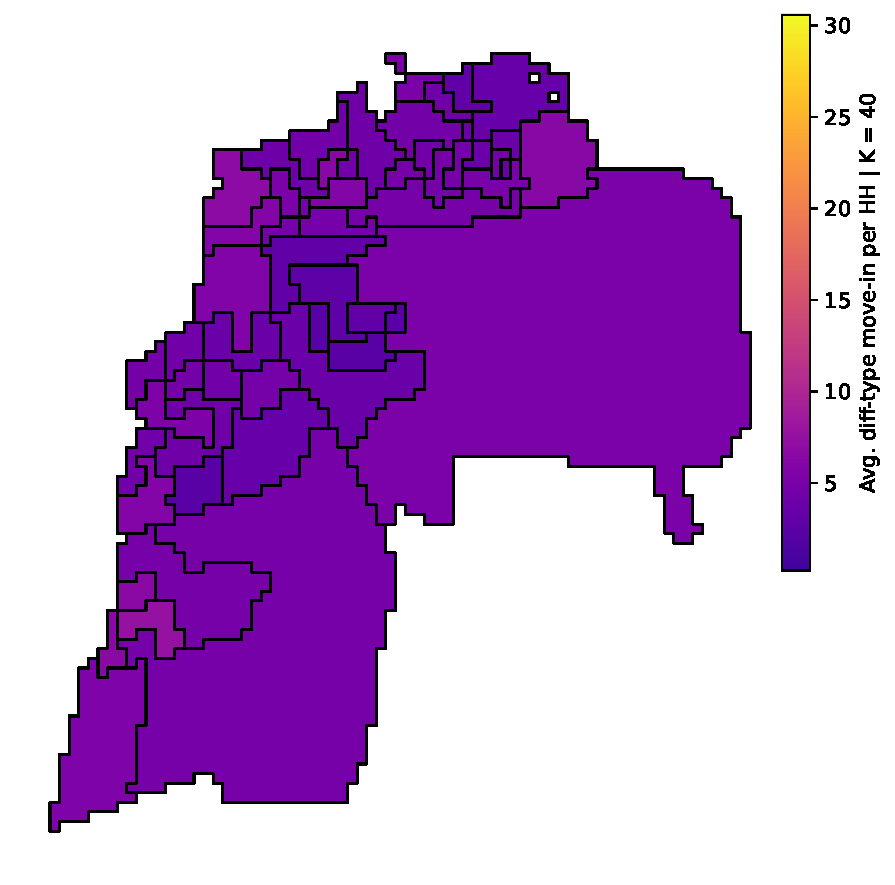
\includegraphics[width=\textwidth]{figs/ishoj_howdy_neighbor.pdf}	
	\caption{Ishøj}
	\end{subfigure}
    \begin{subfigure}{.42\textwidth}	
	\centering
	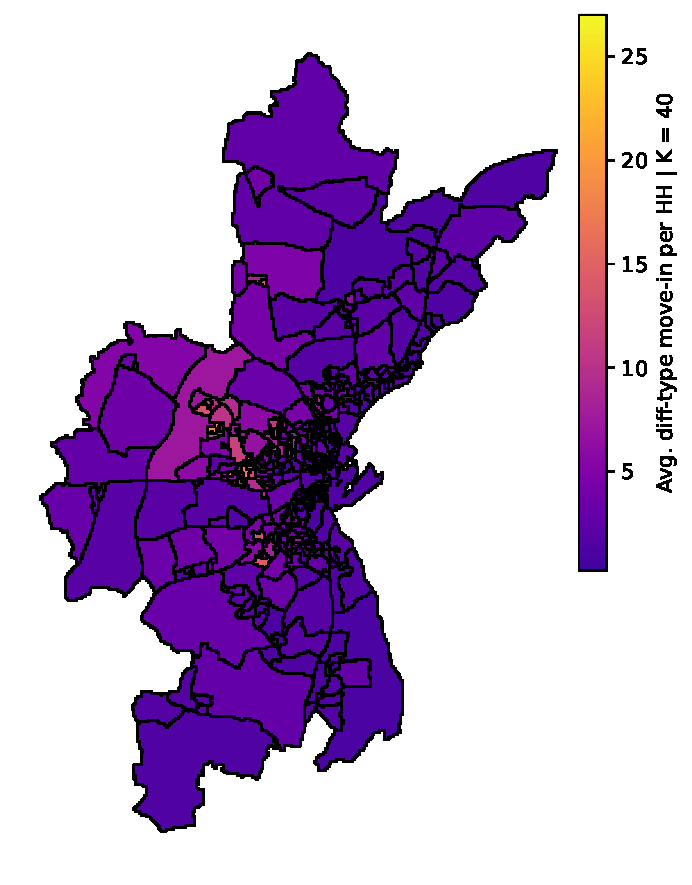
\includegraphics[width=\textwidth]{figs/aarhus_howdy_neighbor.pdf}	
	\caption{Aarhus}
	\end{subfigure}
    
    \begin{subfigure}{.65\textwidth}	
	\centering
	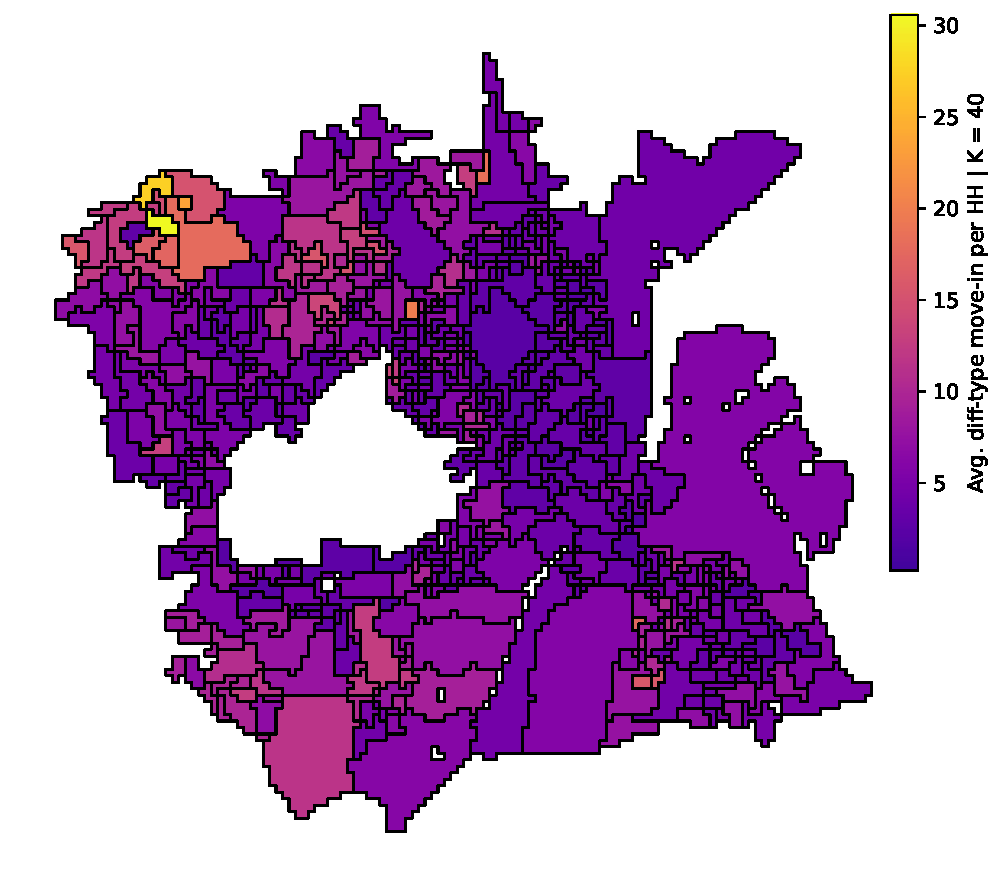
\includegraphics[width=\textwidth]{figs/cph_howdy_neighbor.pdf}	
	\caption{Copenhagen}
	\end{subfigure}	
\begin{tablenotes}
\item \footnotesize \textit{Note:} The figure show the variation in receiving a new-non West neighbor for native households at the \textit{neighborhood} scale for three different municipalities. Neighborhoods not in the sample are greyed out. Household types are split up in three types (native/non-West/West), see section \ref{sec:intro_definitions} for more details. Neighborhoods are defined in section \ref{sec:data_geospatial}. 
\end{tablenotes}
\label{fig:incidence_new_non_west_neighbors_unconstrained}
\end{figure}

\section{The Schelling Model}

\label{sec:appendix_schelling_model_simulation}

Consider a stylized example of Schelling's residential model: 
An $N \times N$ matrix $\textbf{M}$ represents possible residential locations. Two types af agents $b, r$, graphically depicted as blue and red, respectively, are initially allocated a random location within this grid. Agents can differ in terms of ethnicity, income, culture etc. 

The ratio between the two types of agents is constant $N_{b/r} = \frac{N_b}{N_r}$. Further, a constant share of residential locations are vacant, such that $N_{vacant} = N^2 - (N_b + N_r)$. 

Each agent $i = b, r$ "optimizes" their residential location by the share, $s_i$, of their nearest neighbors, who is of the same type. That is, for $s_i \leq \tau$, where a $\tau$ is a fixed global tolerance parameter for the maximum share of neighbours of a different type, each agent $i$ will move until this condition is satisified. 

This is a somewhat stylized version of the Schelling model, though it accurately depicts the model dynamics... Something about the Schelling model... 

Below is a parameterization of the model described above such that red(?) is always in the minority\footnote{This implementation closely follows \textcite{luca_mingarelli}, who very kindly made his code publicly available.}:

\begin{table}[H]
    \centering
    \caption{Schelling model parameters}
    \begin{tabular}{lc}
    \toprule
      Parameter & Value \\
    \midrule
      $N$         & 100 \\
      $N_r$       & 1.25 \\
      $N_{vacant}$ & 0.1 \\
    \bottomrule
    \end{tabular}
\end{table}

For agents $i, j$, suppose they are numerically represented as $i_{red}=1$, $j_{blue} = 0$ with vacant locations $m_v=-1$ in $\textbf{M}$. We can perform element-wise multiplication and summation for each agent in $M$ to determine whether or not this satisfies the condition $s_i \leq \tau$. This process is called convolution and the operation can be done via the following kernel $\mathbf{K}$:

\newpage
\begin{lstlisting}[style=pythonstyle]
import numpy as np
KERNEL = np.array([[1,1,1,1,1],
                   [1,1,1,1,1],
                   [1,1,0,1,1],
                   [1,1,1,1,1],
                   [1,1,1,1,1]])

\end{lstlisting}

With the convolution operation defined as:

\begin{equation}
(K \star M)_{i, j}=\sum_{\substack{a \in\left\{-k_x, \ldots, k_x\right\} \\ b \in\left\{-k_y, \ldots, k_y\right\}}} K_{a+k_x, b+k_y} M_{i+a, j+b}
\label{eq:convolution}
\end{equation}

Where $k_x, k_y \in \mathbb{N}_0$. 


That is, I am considering the $k=24$ nearest neighbors in reference to the tolerance parameter $\tau$.

\begin{figure}[H]
\centering
\caption{Schelling model simulations}
	\begin{subfigure}{0.45\textwidth}	
	\centering
    \caption{Integrated society, $1-\tau = 0.25$}
	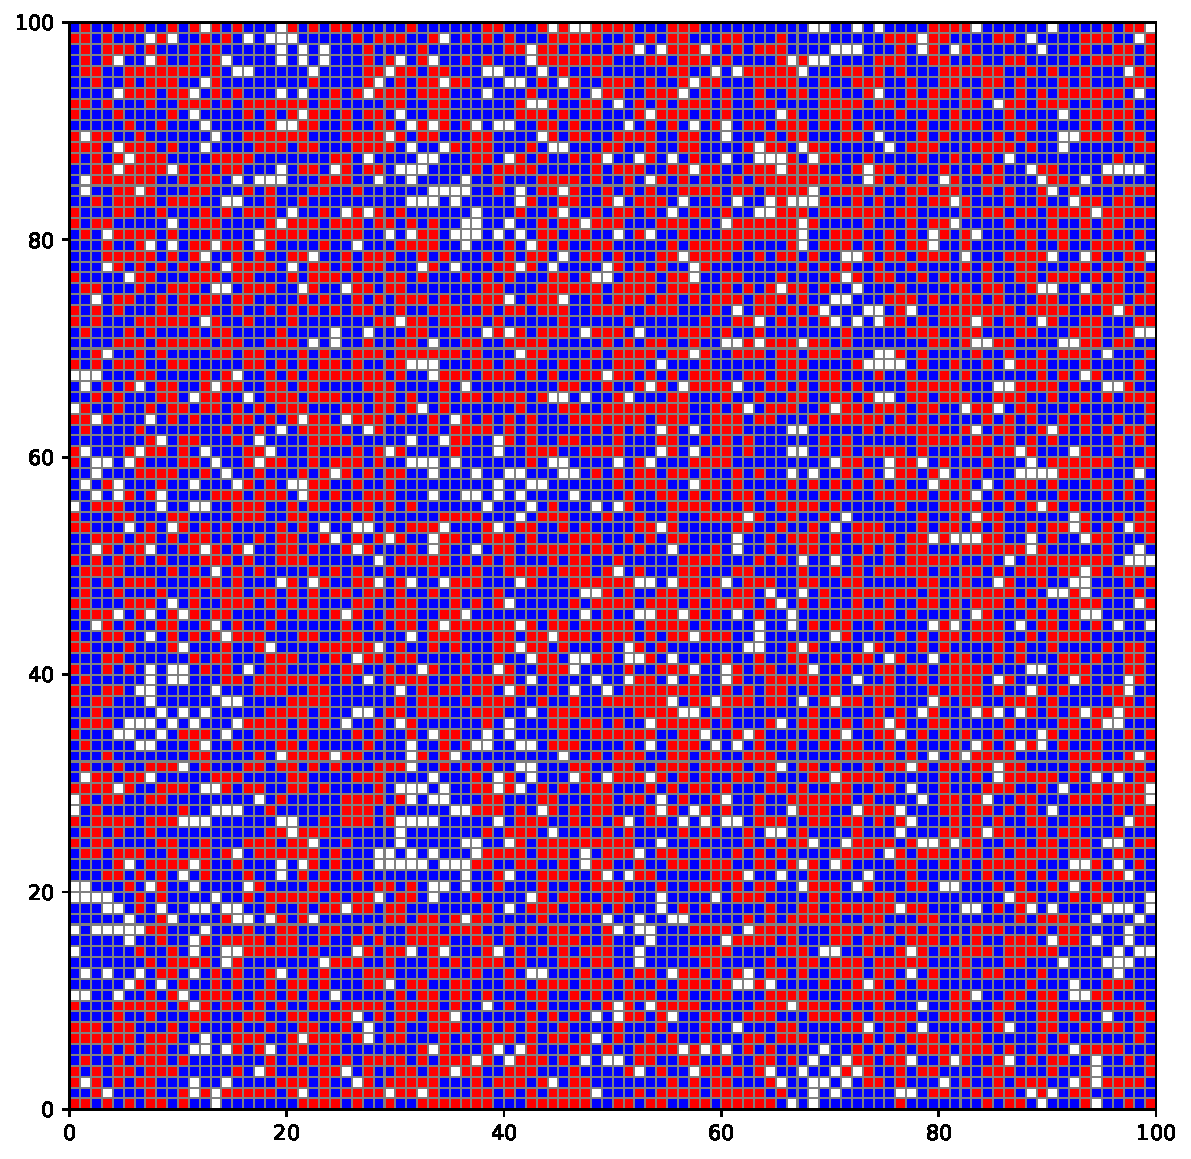
\includegraphics[width=\textwidth]{figs/schelling_model_0.25.pdf}	
	\end{subfigure}	
	\begin{subfigure}{0.45\textwidth}	
	\centering
    \caption{Inbetween(?) society, $1-\tau = 0.33$}
	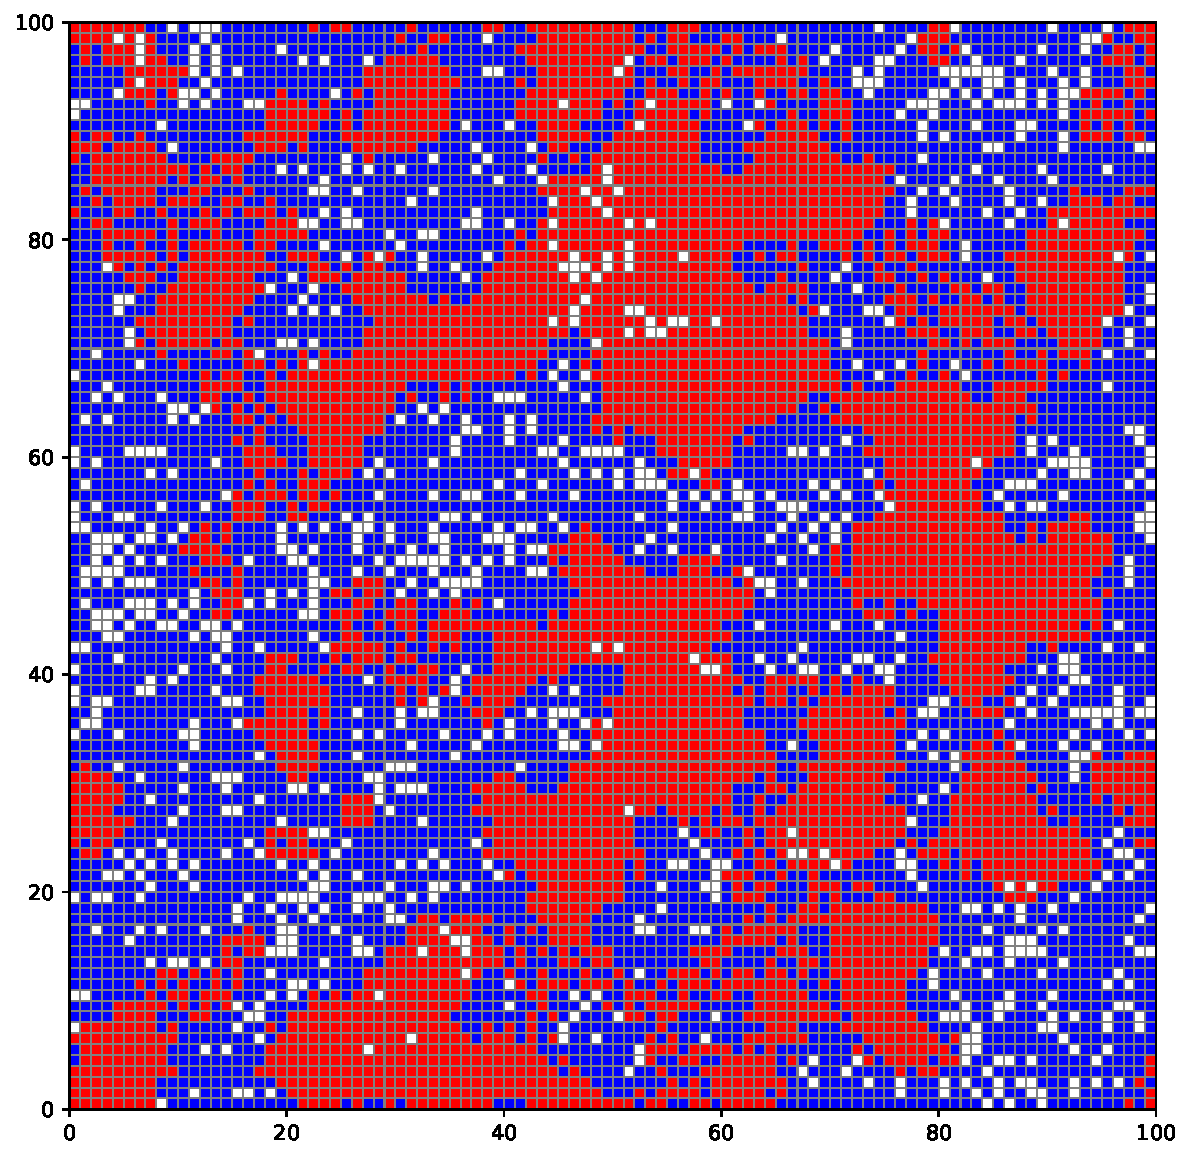
\includegraphics[width=\textwidth]{figs/schelling_model_0.33.pdf}	
	\end{subfigure}	
	\begin{subfigure}{0.45\textwidth}	
	\centering
     \caption{Segregated society, $1-\tau = 0.40$}
	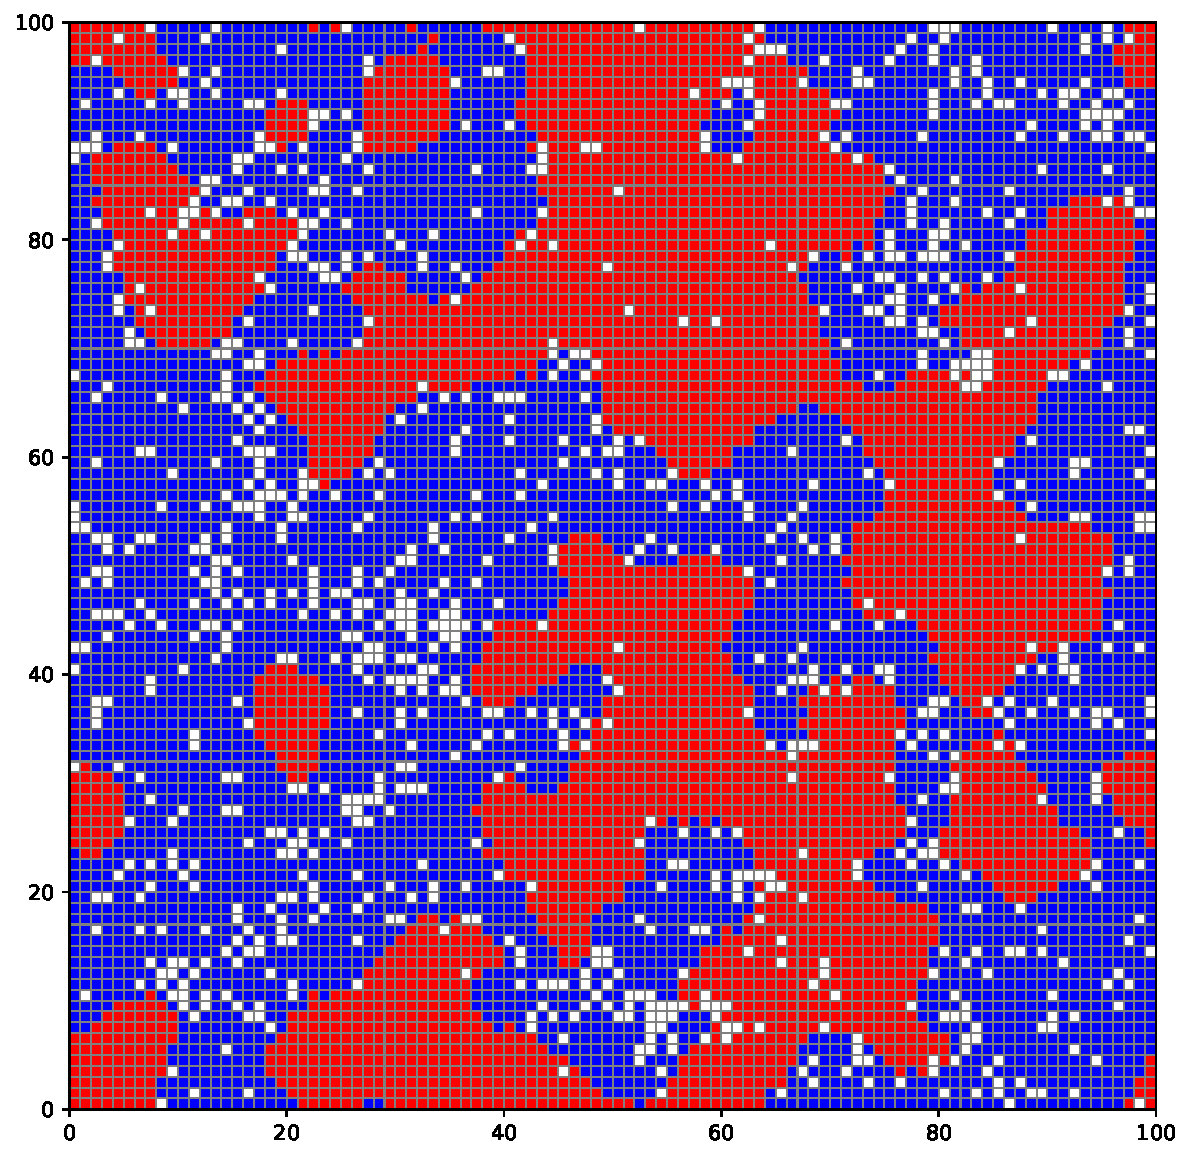
\includegraphics[width=\textwidth]{figs/schelling_model_0.4.pdf}	
	\end{subfigure}
    \begin{subfigure}{0.45\textwidth}	
	\centering
     \caption{"Gated" community, $1-\tau = 0.60$}
	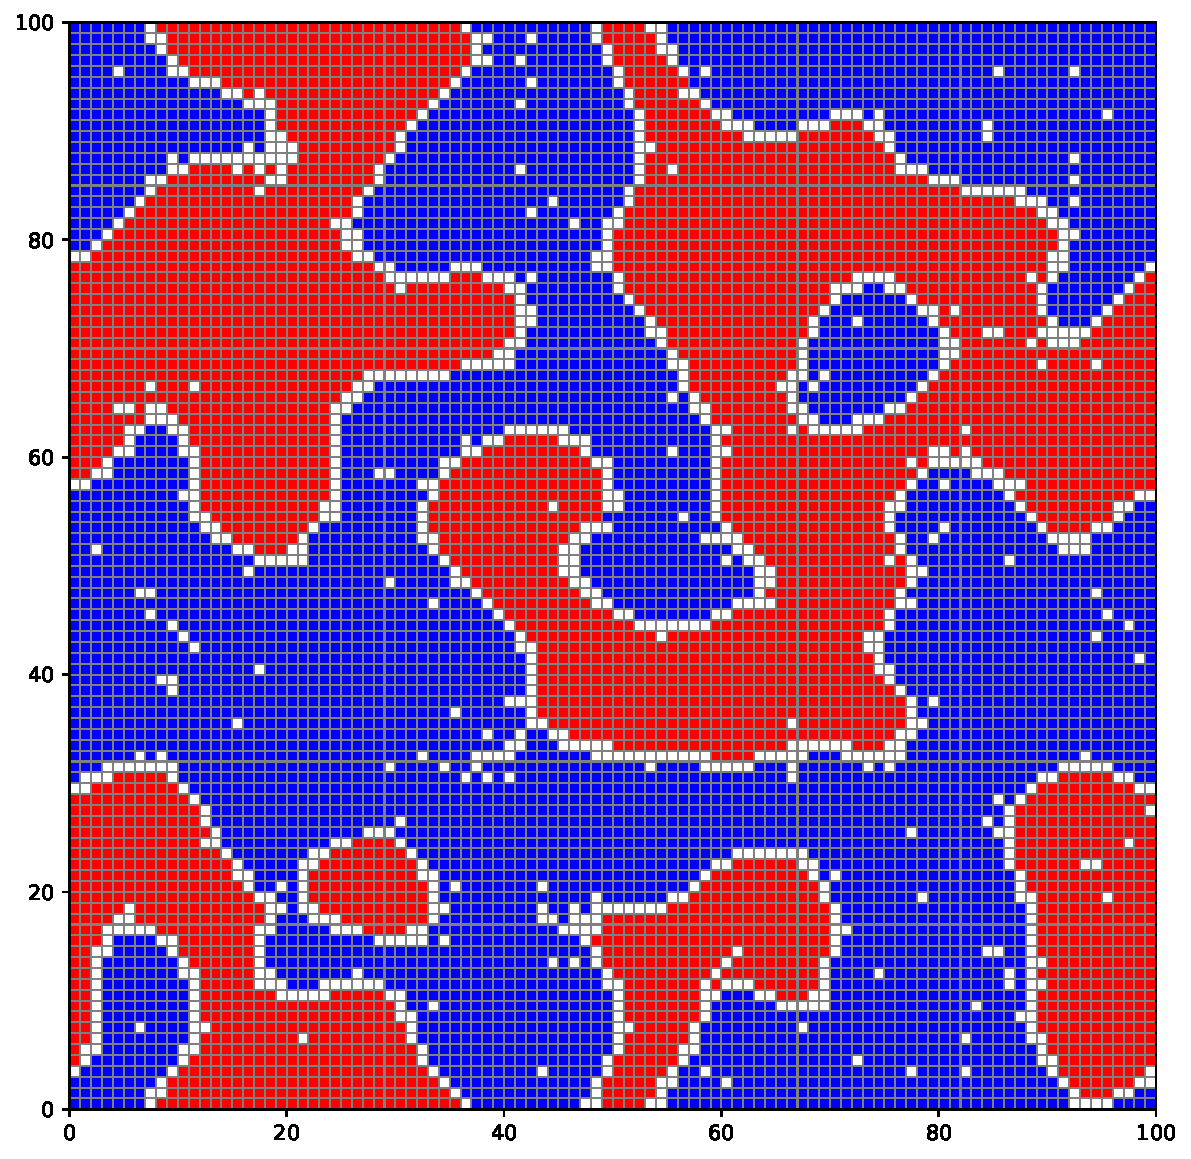
\includegraphics[width=\textwidth]{figs/schelling_model_0.6.pdf}	
	\end{subfigure}
\end{figure}

It is clear that the model predicts a segregated scenario for relatively mild preference parameters. Unsurprisingly, for sufficiently low levels of tolerances, one can observe fairly integrated societies. However, this pattern reverses once the tolerance parameter goes up, but not at levels one might expect. Even when agents are willing to accept up to 60 percent diverse neighbours ($1-\tau = 0.4$), we start to observe almost perfectly segregated societies.

...

\section{Datasets used}
\begin{table}[H]
    \centering
    \caption{Datasets}
    \begin{tabular}{l|p{0.6\linewidth}|c}
    \toprule
      Name & Notes & years \\
    \midrule
      BEF           & The basics, ID, AGE etc               & 1985-2024 \\
      BEFBOP        & Tracks adress changes over time. & 1986-2024 \\
      BEFADR        & Adress register. & 1971-2023 \\
      DAR(?)        & Danish Adress Registry. & 2017-2024 \\ 
      ETRS & (\textbf{NB!}) The "unique" coordinate dataset. & ?-?\\
      EJER & Historical house prices. & 1984-2023 \\
      EJVK & Dwelling valuations. & 1983-2023 \\
      AKM/RAS & (Un)employment. & 1976-2022 \\
      IND & Income, both wage and public transfers. & 1980-2022 \\
      UDDF & Education level. & 1974-2022 \\
      \hdashline
      KRAF(?)       & Crime registry (of court decisions). & 1980-2023\\
      KOTRE(?)      & Completed school grades               & 1970-2023 \\
    \bottomrule
    \end{tabular}
\end{table}

\section{Figures}
\label{sec:appendix_figs}
\begin{figure}[H]
    \centering
    \caption{Neighborhood population share by year}
    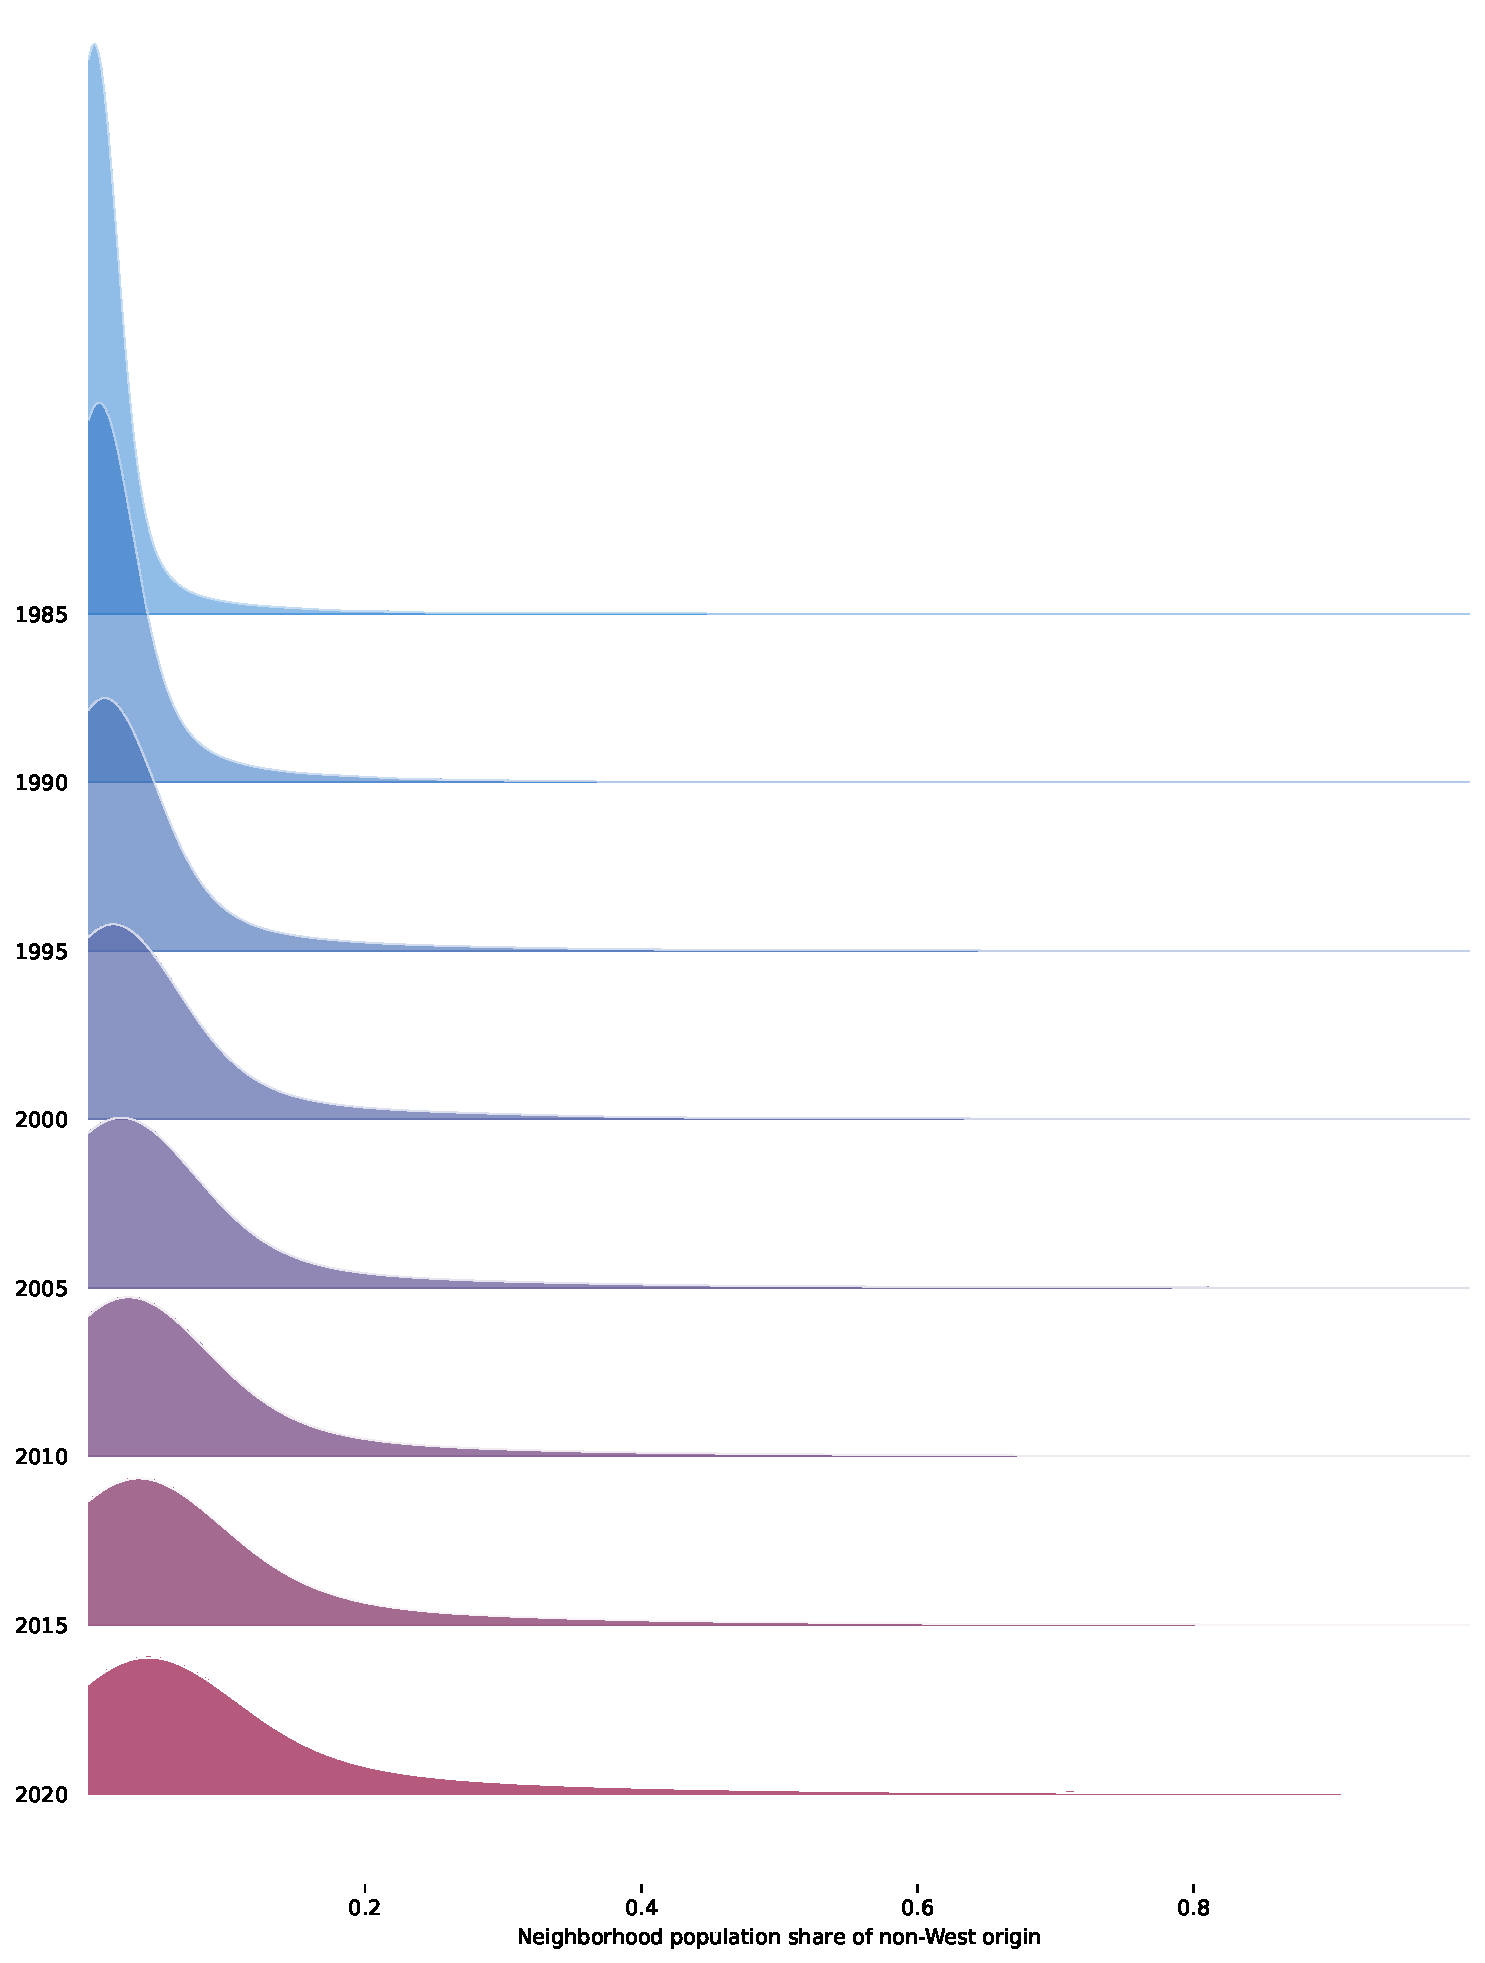
\includegraphics[width=0.7\linewidth]{figs/neighborhood_non_west_share_density_1985_2000.pdf}
        \begin{minipage}{.9\linewidth}
        \footnotesize \textit{Note}: Neighborhoods are derived from \href{https://www.nabolagsatlas.dk/}{Nabolagsatlas}. 
    \end{minipage}
\end{figure}

\begin{figure}[H]
    \centering
    \caption{K = 20 nearest }
    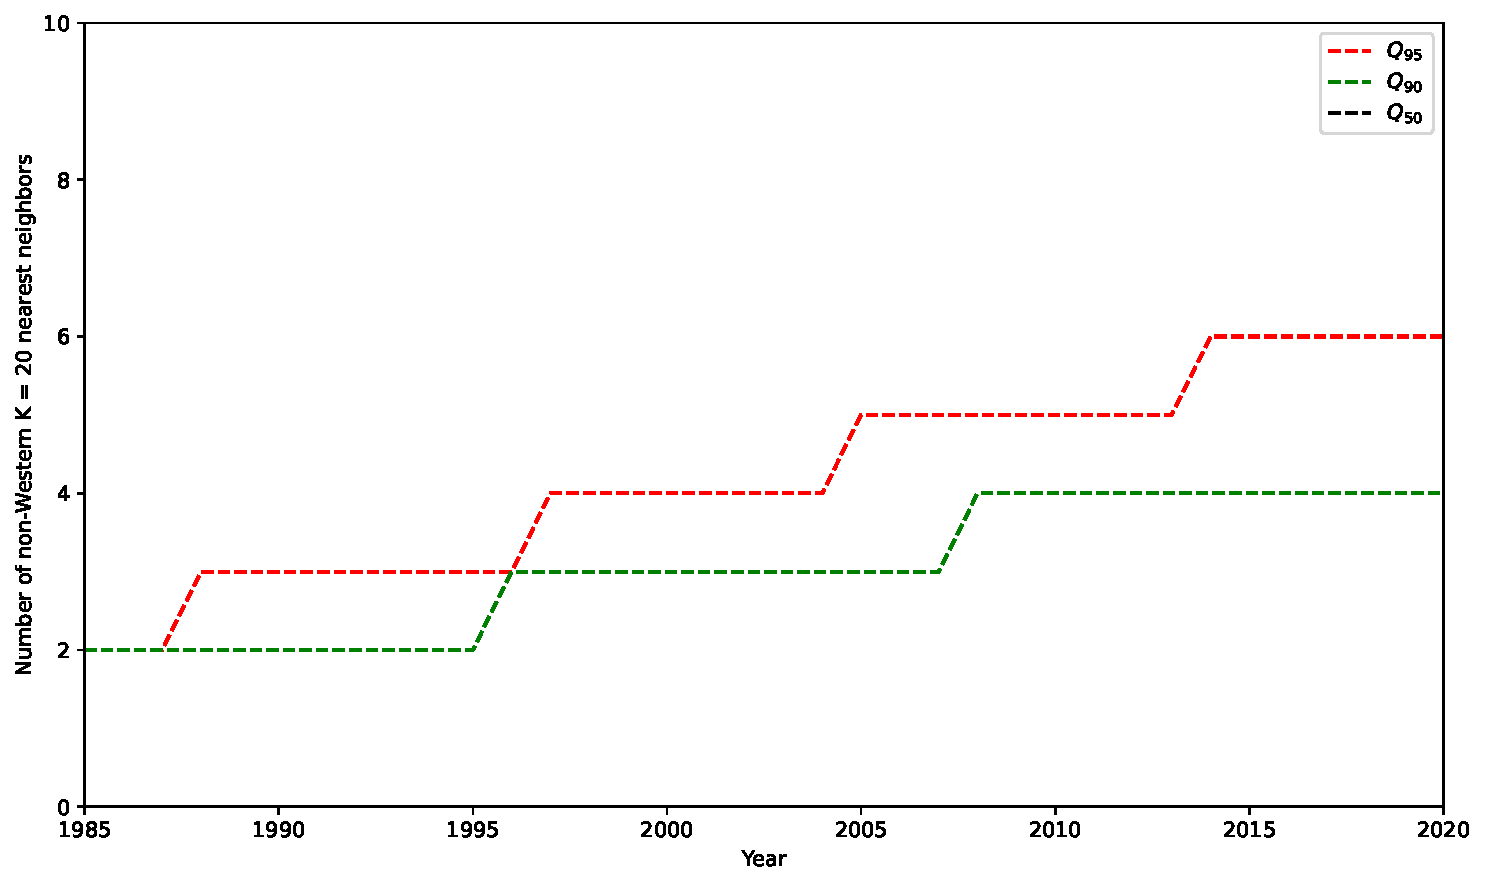
\includegraphics[width=0.7\linewidth]{figs/mix_non_west_pos_nn_quantiles_1985_2020.pdf}
        \begin{minipage}{.7\linewidth}
        \footnotesize \textit{Note}: Non-Western households refers to households where at least one household member is of non-Western origin.
    \end{minipage}
\end{figure}

\end{document}